% ============================================================
% Question Bank: ch02-06 Simple Interest (Modified — FL/TX)
% Topic Title: Simple Interest: Earning and Paying Interest (Financial literacy emphasis)
% CCSS: 7.RP.A.3 (Modified)
% Questions: 30 (18 MC + 7 SA + 5 Graphical)
% ============================================================

% --- Multiple Choice Questions (18) ---

\begin{practiceQuestion}{m-2-6-q01}{mc}
\begin{questionText}
What is the simple interest earned on $\$500$ at $4\%$ for $3$ years?
\end{questionText}
\choiceA{$\$6$}
\choiceB{$\$20$}
\choiceC{$\$60$}
\choiceD{$\$600$}
\correctAnswer{C}
\explanation{$I = Prt = 500 \times 0.04 \times 3 = \$60$.}
\end{practiceQuestion}

\begin{practiceQuestion}{m-2-6-q02}{mc}
\begin{questionText}
You borrow $\$2{,}000$ at $5\%$ simple interest for $2$ years. What is the total amount you owe?
\end{questionText}
\choiceA{$\$200$}
\choiceB{$\$2{,}100$}
\choiceC{$\$2{,}200$}
\choiceD{$\$2{,}500$}
\correctAnswer{C}
\explanation{$I = 2{,}000 \times 0.05 \times 2 = \$200$. Total: $2{,}000 + 200 = \$2{,}200$.}
\end{practiceQuestion}

\begin{practiceQuestion}{m-2-6-q03}{mc}
\begin{questionText}
In the formula $I = Prt$, what does $P$ represent?
\end{questionText}
\choiceA{The interest earned}
\choiceB{The percent rate}
\choiceC{The principal (starting amount)}
\choiceD{The time in months}
\correctAnswer{C}
\explanation{$P$ stands for the principal — the original amount of money deposited or borrowed.}
\end{practiceQuestion}

\begin{practiceQuestion}{m-2-6-q04}{mc}
\begin{questionText}
Bank~A offers $3\%$ simple interest. Bank~B offers $5\%$ simple interest. You deposit $\$1{,}000$ for $2$ years. How much more does Bank~B earn?
\end{questionText}
\choiceA{$\$20$}
\choiceB{$\$40$}
\choiceC{$\$60$}
\choiceD{$\$100$}
\correctAnswer{B}
\explanation{Bank A: $1{,}000 \times 0.03 \times 2 = \$60$. Bank B: $1{,}000 \times 0.05 \times 2 = \$100$. Difference: $100 - 60 = \$40$.}
\end{practiceQuestion}

\begin{practiceQuestion}{m-2-6-q05}{mc}
\begin{questionText}
A student calculates: $I = 800 \times 6 \times 3 = \$14{,}400$. What error did the student make?
\end{questionText}
\choiceA{Used the wrong formula}
\choiceB{Forgot to convert $6\%$ to a decimal}
\choiceC{Switched $P$ and $t$}
\choiceD{Divided instead of multiplied}
\correctAnswer{B}
\explanation{$6\%$ must be written as $0.06$. Correct: $I = 800 \times 0.06 \times 3 = \$144$, not $\$14{,}400$.}
\end{practiceQuestion}

\begin{practiceQuestion}{m-2-6-q06}{mc}
\begin{questionText}
A loan of $\$3{,}000$ charges $\$450$ in interest over $3$ years. What is the annual interest rate?
\end{questionText}
\choiceA{$3\%$}
\choiceB{$4\%$}
\choiceC{$5\%$}
\choiceD{$15\%$}
\correctAnswer{C}
\explanation{$450 = 3{,}000 \times r \times 3$. So $9{,}000r = 450$ and $r = 0.05 = 5\%$.}
\end{practiceQuestion}

\begin{practiceQuestion}{m-2-6-q07}{mc}
\begin{questionText}
You want to earn $\$200$ in interest on a $\$2{,}500$ deposit at $4\%$ simple interest. How many years do you need to save?
\end{questionText}
\choiceA{$1$ year}
\choiceB{$2$ years}
\choiceC{$3$ years}
\choiceD{$5$ years}
\correctAnswer{B}
\explanation{$200 = 2{,}500 \times 0.04 \times t$. So $100t = 200$ and $t = 2$ years.}
\end{practiceQuestion}

\begin{practiceQuestion}{m-2-6-q08}{mc}
\begin{questionText}
Which deposit earns the most interest: $\$600$ at $5\%$ for $2$ years, or $\$600$ at $3\%$ for $4$ years?
\end{questionText}
\choiceA{$5\%$ for $2$ years — $\$60$}
\choiceB{$3\%$ for $4$ years — $\$72$}
\choiceC{They earn the same}
\choiceD{$5\%$ for $2$ years — $\$100$}
\correctAnswer{B}
\explanation{Option 1: $600 \times 0.05 \times 2 = \$60$. Option 2: $600 \times 0.03 \times 4 = \$72$. The longer time at a lower rate earns more.}
\end{practiceQuestion}

\begin{practiceQuestion}{m-2-6-q09}{mc}
\begin{questionText}
You deposit $\$1{,}500$ at $2.5\%$ simple interest for $4$ years. What is the total amount in the account?
\end{questionText}
\choiceA{$\$1{,}515$}
\choiceB{$\$1{,}550$}
\choiceC{$\$1{,}600$}
\choiceD{$\$1{,}650$}
\correctAnswer{D}
\explanation{$I = 1{,}500 \times 0.025 \times 4 = \$150$. Total: $1{,}500 + 150 = \$1{,}650$.}
\end{practiceQuestion}

\begin{practiceQuestion}{m-2-6-q10}{mc}
\begin{questionText}
A car loan is $\$8{,}000$ at $6\%$ simple interest for $5$ years. How much interest is paid over the life of the loan?
\end{questionText}
\choiceA{$\$240$}
\choiceB{$\$480$}
\choiceC{$\$2{,}400$}
\choiceD{$\$4{,}800$}
\correctAnswer{C}
\explanation{$I = 8{,}000 \times 0.06 \times 5 = \$2{,}400$.}
\end{practiceQuestion}

\begin{practiceQuestion}{m-2-6-q11}{mc}
\begin{questionText}
When you save money in a bank, the bank pays you interest. When you borrow money, you pay the bank interest. Which scenario means you owe \textbf{more} than you borrowed?
\end{questionText}
\choiceA{Depositing money in savings}
\choiceB{Taking out a loan}
\choiceC{Earning interest on a CD}
\choiceD{Putting money in a checking account}
\correctAnswer{B}
\explanation{When you borrow, the interest is added to what you owe. You pay back more than you originally borrowed.}
\end{practiceQuestion}

\begin{practiceQuestion}{m-2-6-q12}{mc}
\begin{questionText}
Loan~A: $\$1{,}000$ at $8\%$ for $2$ years. Loan~B: $\$1{,}000$ at $4\%$ for $3$ years. Which loan charges less total interest?
\end{questionText}
\choiceA{Loan A — $\$160$}
\choiceB{Loan B — $\$120$}
\choiceC{They charge the same}
\choiceD{Loan A — $\$80$}
\correctAnswer{B}
\explanation{Loan A: $1{,}000 \times 0.08 \times 2 = \$160$. Loan B: $1{,}000 \times 0.04 \times 3 = \$120$. Loan B costs less.}
\end{practiceQuestion}

\begin{practiceQuestion}{m-2-6-q13}{mc}
\begin{questionText}
An account earns $\$180$ in simple interest. The rate is $3\%$ and the time is $4$ years. What was the principal?
\end{questionText}
\choiceA{$\$1{,}200$}
\choiceB{$\$1{,}500$}
\choiceC{$\$2{,}160$}
\choiceD{$\$6{,}000$}
\correctAnswer{B}
\explanation{$180 = P \times 0.03 \times 4 = 0.12P$. So $P = 180 \div 0.12 = \$1{,}500$.}
\end{practiceQuestion}

\begin{practiceQuestion}{m-2-6-q14}{mc}
\begin{questionText}
You deposit $\$400$ at $6\%$ simple interest. After how many years will the interest equal the original deposit?
\end{questionText}
\choiceA{About $6$ years}
\choiceB{About $10$ years}
\choiceC{About $17$ years}
\choiceD{It will never happen}
\correctAnswer{C}
\explanation{$400 = 400 \times 0.06 \times t = 24t$. So $t = 400 \div 24 \approx 16.7$ years, which is about $17$ years.}
\end{practiceQuestion}

\begin{practiceQuestion}{m-2-6-q15}{mc}
\begin{questionText}
Which change would increase the interest earned the most: doubling $P$, doubling $r$, or doubling $t$?
\end{questionText}
\choiceA{Doubling $P$}
\choiceB{Doubling $r$}
\choiceC{Doubling $t$}
\choiceD{All three changes give the same increase}
\correctAnswer{D}
\explanation{Since $I = Prt$, doubling any one factor doubles the interest. All three changes have the same effect.}
\end{practiceQuestion}

\begin{practiceQuestion}{m-2-6-q16}{mc}
\begin{questionText}
A savings account has $\$750$ at $2\%$ for $5$ years. What is the interest earned?
\end{questionText}
\choiceA{$\$7.50$}
\choiceB{$\$37.50$}
\choiceC{$\$75$}
\choiceD{$\$750$}
\correctAnswer{C}
\explanation{$I = 750 \times 0.02 \times 5 = \$75$.}
\end{practiceQuestion}

\begin{practiceQuestion}{m-2-6-q17}{mc}
\begin{questionText}
A loan charges $\$360$ interest on $\$2{,}400$ over $2$ years. What is the annual rate?
\end{questionText}
\choiceA{$6\%$}
\choiceB{$7.5\%$}
\choiceC{$10\%$}
\choiceD{$15\%$}
\correctAnswer{B}
\explanation{$360 = 2{,}400 \times r \times 2 = 4{,}800r$. So $r = 360 \div 4{,}800 = 0.075 = 7.5\%$.}
\end{practiceQuestion}

\begin{practiceQuestion}{m-2-6-q18}{mc}
\begin{questionText}
You borrow $\$5{,}000$ at $4.5\%$ for $3$ years. What is the total you must repay?
\end{questionText}
\choiceA{$\$5{,}225$}
\choiceB{$\$5{,}450$}
\choiceC{$\$5{,}675$}
\choiceD{$\$6{,}350$}
\correctAnswer{C}
\explanation{$I = 5{,}000 \times 0.045 \times 3 = \$675$. Total: $5{,}000 + 675 = \$5{,}675$.}
\end{practiceQuestion}

% --- Short Answer Questions (7) ---

\begin{practiceQuestion}{m-2-6-q19}{sa}
\begin{questionText}
You deposit $\$900$ at $3\%$ simple interest for $5$ years. How much interest do you earn?
\end{questionText}
\correctAnswer{$\$135$}
\explanation{$I = 900 \times 0.03 \times 5 = \$135$.}
\end{practiceQuestion}

\begin{practiceQuestion}{m-2-6-q20}{sa}
\begin{questionText}
A loan of $\$4{,}000$ at $7\%$ simple interest for $3$ years charges how much interest?
\end{questionText}
\correctAnswer{$\$840$}
\explanation{$I = 4{,}000 \times 0.07 \times 3 = \$840$.}
\end{practiceQuestion}

\begin{practiceQuestion}{m-2-6-q21}{sa}
\begin{questionText}
You want to earn $\$100$ in interest on $\$2{,}000$ at $2.5\%$ simple interest. How many years must you save?
\end{questionText}
\correctAnswer{$2$ years}
\explanation{$100 = 2{,}000 \times 0.025 \times t = 50t$. So $t = 100 \div 50 = 2$ years.}
\end{practiceQuestion}

\begin{practiceQuestion}{m-2-6-q22}{sa}
\begin{questionText}
An account earned $\$270$ in simple interest at $6\%$ over $3$ years. What was the principal?
\end{questionText}
\correctAnswer{$\$1{,}500$}
\explanation{$270 = P \times 0.06 \times 3 = 0.18P$. So $P = 270 \div 0.18 = \$1{,}500$.}
\end{practiceQuestion}

\begin{practiceQuestion}{m-2-6-q23}{sa}
\begin{questionText}
A $\$3{,}500$ loan at $4\%$ charges $\$280$ in interest. How many years is the loan?
\end{questionText}
\correctAnswer{$2$ years}
\explanation{$280 = 3{,}500 \times 0.04 \times t = 140t$. So $t = 280 \div 140 = 2$ years.}
\end{practiceQuestion}

\begin{practiceQuestion}{m-2-6-q24}{sa}
\begin{questionText}
Account~A: $\$1{,}000$ at $4\%$ for $5$ years. Account~B: $\$1{,}000$ at $5\%$ for $4$ years. Which earns more interest, and by how much?
\end{questionText}
\correctAnswer{They are equal — both earn $\$200$}
\explanation{A: $1{,}000 \times 0.04 \times 5 = \$200$. B: $1{,}000 \times 0.05 \times 4 = \$200$. They earn the same amount.}
\end{practiceQuestion}

\begin{practiceQuestion}{m-2-6-q25}{sa}
\begin{questionText}
You deposit $\$2{,}500$ at $3.5\%$ for $4$ years. What is the total amount in the account at the end?
\end{questionText}
\correctAnswer{$\$2{,}850$}
\explanation{$I = 2{,}500 \times 0.035 \times 4 = \$350$. Total: $2{,}500 + 350 = \$2{,}850$.}
\end{practiceQuestion}

% --- Graphical Questions (3 GMC + 2 GSA) ---

\begin{practiceQuestion}{m-2-6-q26}{gmc}
\begin{questionText}
The table shows two bank offers. Which earns more interest on a $\$1{,}000$ deposit for $3$ years?

\begin{center}
\begin{tabular}{|l|c|c|}
\hline
 & \textbf{Rate} & \textbf{Time} \\
\hline
Bank A & $3.5\%$ & $3$ years \\
\hline
Bank B & $2\%$ & $3$ years \\
\hline
\end{tabular}
\end{center}
\end{questionText}
\choiceA{Bank A — $\$105$}
\choiceB{Bank B — $\$60$}
\choiceC{Bank A — $\$35$}
\choiceD{They earn the same}
\correctAnswer{A}
\explanation{Bank A: $1{,}000 \times 0.035 \times 3 = \$105$. Bank B: $1{,}000 \times 0.02 \times 3 = \$60$. Bank A earns more.}
\end{practiceQuestion}

\begin{practiceQuestion}{m-2-6-q27}{gmc}
\begin{questionText}
The bar graph shows the interest earned on two accounts over $4$ years.

\begin{center}
\begin{tikzpicture}[scale=0.6]
  \draw[thick,->] (0,0) -- (0,7) node[above]{\footnotesize Interest (\$)};
  \draw[thick,->] (0,0) -- (7,0);
  % Bars
  \fill[funBlue!60] (1,0) rectangle (2.5,4);
  \fill[funOrange!60] (3.5,0) rectangle (5,5.6);
  \node[below] at (1.75,0) {\footnotesize Acct A};
  \node[below] at (4.25,0) {\footnotesize Acct B};
  % Y-axis labels
  \foreach \y/\val in {0/0, 1/50, 2/100, 3/150, 4/200, 5/250, 6/300} {
    \draw(-0.15,\y) -- (0.15,\y);
    \node[left] at (-0.15,\y) {\footnotesize $\$\val$};
  }
  \node[above] at (1.75,4) {\footnotesize $\$200$};
  \node[above] at (4.25,5.6) {\footnotesize $\$280$};
\end{tikzpicture}
\end{center}

Both accounts started with $\$1{,}000$. What is the annual rate for Account A?
\end{questionText}
\choiceA{$4\%$}
\choiceB{$5\%$}
\choiceC{$6\%$}
\choiceD{$7\%$}
\correctAnswer{B}
\explanation{$200 = 1{,}000 \times r \times 4$. So $4{,}000r = 200$ and $r = 0.05 = 5\%$.}
\end{practiceQuestion}

\begin{practiceQuestion}{m-2-6-q28}{gmc}
\begin{questionText}
The timeline shows a savings plan. How much total money is in the account at the end?

\begin{center}
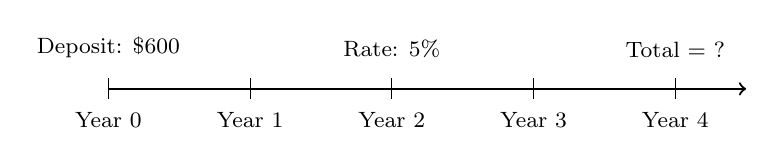
\begin{tikzpicture}[scale=0.9]
  \draw[thick,->] (0,0) -- (9,0);
  \foreach \x/\lab in {0/Year 0, 2/Year 1, 4/Year 2, 6/Year 3, 8/Year 4} {
    \draw (\x,0.15) -- (\x,-0.15);
    \node[below] at (\x,-0.2) {\footnotesize \lab};
  }
  \node[above] at (0,0.3) {\footnotesize Deposit: $\$600$};
  \node[above] at (4,0.3) {\footnotesize Rate: $5\%$};
  \node[above] at (8,0.3) {\footnotesize Total = ?};
\end{tikzpicture}
\end{center}
\end{questionText}
\choiceA{$\$620$}
\choiceB{$\$680$}
\choiceC{$\$720$}
\choiceD{$\$750$}
\correctAnswer{C}
\explanation{$I = 600 \times 0.05 \times 4 = \$120$. Total: $600 + 120 = \$720$.}
\end{practiceQuestion}

\begin{practiceQuestion}{m-2-6-q29}{gsa}
\begin{questionText}
Complete the table for a $\$2{,}000$ deposit at $3\%$ simple interest.

\begin{center}
\begin{tabular}{|c|c|c|}
\hline
\textbf{Year} & \textbf{Interest Earned (Total)} & \textbf{Account Balance} \\
\hline
$0$ & $\$0$ & $\$2{,}000$ \\
\hline
$1$ & $\$60$ & $\$2{,}060$ \\
\hline
$2$ & ? & ? \\
\hline
$3$ & ? & ? \\
\hline
\end{tabular}
\end{center}
\end{questionText}
\correctAnswer{Year 2: $\$120$, $\$2{,}120$; Year 3: $\$180$, $\$2{,}180$}
\explanation{Each year earns $2{,}000 \times 0.03 = \$60$. Year 2: total interest $= \$120$, balance $= \$2{,}120$. Year 3: total interest $= \$180$, balance $= \$2{,}180$.}
\end{practiceQuestion}

\begin{practiceQuestion}{m-2-6-q30}{gsa}
\begin{questionText}
The table compares two loan options for borrowing $\$5{,}000$. Find the total cost (principal + interest) for each loan.

\begin{center}
\begin{tabular}{|l|c|c|c|}
\hline
 & \textbf{Principal} & \textbf{Rate} & \textbf{Time} \\
\hline
Loan A & $\$5{,}000$ & $3\%$ & $5$ years \\
\hline
Loan B & $\$5{,}000$ & $6\%$ & $3$ years \\
\hline
\end{tabular}
\end{center}

Which loan costs less overall?
\end{questionText}
\correctAnswer{Loan A: $\$5{,}750$; Loan B: $\$5{,}900$; Loan A costs less}
\explanation{Loan A: $I = 5{,}000 \times 0.03 \times 5 = \$750$. Total: $\$5{,}750$. Loan B: $I = 5{,}000 \times 0.06 \times 3 = \$900$. Total: $\$5{,}900$. Loan A saves $\$150$.}
\end{practiceQuestion}
